\documentclass[12pt]{article}
\usepackage{fontspec}
\setmainfont{Times New Roman}
\usepackage[legalpaper,margin=0.8in]{geometry}
\usepackage{xcolor}
\usepackage{amsmath}
\usepackage{graphicx}
\usepackage{caption}
\usepackage{longtable} % For long tables spanning multiple pages
\usepackage{array}
\usepackage{makecell}
\usepackage{setspace}
\onehalfspacing % Για απόσταση 1.5 γραμμών
\usepackage{pgfplots}
\pgfplotsset{compat=1.17}
\usepackage{pgfplotstable} 
\usepackage{booktabs}

\title{Η απόδοση των μαθητών λαμβάνοντας υπόψη παράγοντες της καθημερινότητας τους}




\author{Ιωάννου Νικόλας - ge20718 
\\ Μπέκος Θοδωρής - ge}
\date{Δεκέμβριος 2024}


\begin{document}
\maketitle

\vspace{0.7cm}
\begin{center}
    
\includegraphics[width=0.7\textwidth]{./images/Εθνικό_Μετσόβειο_Πολυτεχνείο.svg}
    
    \Large Σχολή εφαρμοσμένων μαθηματικών και φυσικών επιστημών \\[1.5cm]
\end{center}



        
\vfill


        \noindent Μάθημα: ΘΕΜΑ \\[0.5cm]


        \noindent\textbf{Υπέυθυνος καθηγητής:} 
        Δρ. Στεφανέας Πέτρος \\[1cm]

\newpage
\noindent\textbf{Ευχαριστίες:} \\

\noindent Θα θέλαμε να ευχαριστήσουμε τον κύριο Πέτρο Στεφανέα για το ενδιαφέρον και
την εμπιστοσύνη που μας έδειξε κατά τη διάρκεια πραγματοποίησης της εν λόγω εργασίας. Επίσης, θα θέλαμε να ευχαριστήσουμε τις οικογένειες μας γιατί χωρίς αυτές δεν θα μπορούσαμε να βρισκόμασταν στη θέση που βρισκόμαστε τώρα.

\newpage
\renewcommand{\contentsname}{\Huge \textbf{Περιεχόμενα}}

% Πίνακας περιεχομένων
\tableofcontents
\newpage

\section{Εισαγωγή}
km \\
\newpage

\section*{Introduction}
gt \\
\newpage
\section{Ανάλυση της διαδικασίας επιλογής μοντέλου}
\subsection{Ανάλυση του προβλήματος}

\noindent Το πρόβλημα το οποίο αντιμετωπίσαμε είχει να κάνει με την δημιουργία ενός μοντέλου μηχανικής μάθησης για την εκτίμηση των βαθμών που θα επιτύχουν οι μαθητές στην εξέταση ενός μαθήματος , μέσω διαφόρων παραγόντων που θα αναλύσουμε παρακάτω. Το πρόβλημα αυτό αποτελεί πρόβλημα παλινδρόμισης αφού ο τελικός βαθμός δεν αποτελεί κατηγορική αλλά ποσοτική μεταβλητή και παίρνει συνεχείς τιμές. Χρησιμοποιήσαμε το σύνολο δεδομένων  Student Performance Factors που βρήκαμε στο Kaggle, όπου τα χαρακτηριστικά τα οποία το αποτελούν φαίνονται στον πίνακα παρακάτω:\\

\begin{center}
\begin{longtable}{|p{5cm}|p{7.1cm}|p{4cm}|} % Creates a table with 3 columns, all centered, with borders
\hline
Χαρακτηριστικά & Περιγραφή & Εύρος τιμών \\ % Header row
\hline
Attendance & \makecell[l]{Ποσοστό μαθημάτων που\\ παρευρέθηκε ο μαθητής} & 0-100 \\ % Row 1
\hline
Previous Scores & \makecell[l]{Μέσος όρος βαθμών απο\\ προηγούμενες εξετάσεις} & 0-100 \\ % Row 7
\hline
Sleep Hours & \makecell[l]{Ώρες ύπνου ανά μέσο όρο\\ κάθε βράδυ} & 4-10 \\ % Row 6
\hline
Hours Studied & Αριθμός ωρών που δίαβασε ο μαθητής μέσα στην βδομάδα & 0-50 \\ % Row 2
\hline
Tutoring Sessions &\makecell[l]{Αριθμός φροντιστηριακών\\ μαθημάτων ανά μήνα} & 0-10 \\ % Row 10
\hline
Family income & Οικογενειακό εισόδημα & Low/Medium/ High \\ % Row 11
\hline
Teacher quality & \makecell[l]{Εκπαιδευτική ικανότητα\\ καθηγητή} & Low/Medium/ High \\ % Row 12
\hline
\makecell[l]{Parental\\ Involvement} & \makecell[l]{Βαθμός εμπλοκής γονέων\\ στην εκπαίδευση του μαθητή} & Low/Medium/ High \\ % Row 3
\hline
Access to Resources & \makecell[l]{Πρόσβαση μαθητή σε\\ εκπαιδευτικό υλικό} & Low/Medium/ High \\ % Row 4
\hline
Motivation Level & Κίνητρο μαθητή & Low/Medium/ High \\ % Row 8
\hline
Peer Influence & \makecell[l]{Επιρροή που δέχεται ο\\ μαθητής απο ομήλικους του} & \makecell[l]{Negative/\\ Neutral/ \\Positive} \\ % Row 14
\hline
Distance from home & Απόσταση σχολείου απο το σπίτι & Near/Moderate/ Far \\ % Row 18
\hline
School type & Τύπος σχολείου & Private/Public \\ % Row 13
\hline

Physical activity & \makecell[l]{Επίπεδο φυσικής \\ δραστηριότητας μαθητή} & \makecell[l]{Sedentary/ \\ Light/Moderate/ \\ Active/ \\ Very Active/ \\ Highly Active/ \\ Athlete} \\ % Row 15
\hline

\makecell[l]{Parental education \\level} & Επίπεδο εκπαίδευσης γονέα & \makecell[l]{High School/ \\ College/ \\ Postgraduate} \\ % Row 17
\hline
Extracurricular activities & Εξωσχολικές δραστηριότητες & Yes/No \\ % Row 5
\hline
Learning disabilities & Μαθησιακές δυσκολίες & Yes/No \\ % Row 16
\hline

Internet Access & Πρόσβαση στο διαδίκτυο & Yes/No \\ % Row 9
\hline
Gender & Φύλο μαθητή & Male/Female \\ % Row 19
\hline

Exam Score & Βαθμός εξέτασης & 0-100 \\ % Row 20
\hline
\end{longtable}
\end{center}

Η μεταβλητή Exam Score αποτελεί την εξαρτημένη μεταβλητή(μεταβλητή στόχο) του μοντέλου ενώ οι υπόλοιπες μεταβλητές αποτελούν τις πιθανές ανεξάρτητες μεταβλητές. 


\subsection{Επεξεργασία των δεδομένων}
Ρίχνωντας μια ματιά στα δεδομένα παρατηρήσαμε πως υπάρχουν παρατηρήσεις με ελλειπείς τιμές. Στην συγκεκριμένη περίπτωση έχουμε 3 επιλογές. Η πρώτη επιλογή ήταν να διαγράψουμε τις παρατηρήσεις αυτές, η δεύτερη να προβλέψουμε τις τιμές των παρατηρήσεων με κάποια μέθοδο (Παλινδρόμιση για τις ποσοτικές και ομαδοποίηση για της κατηγορικές μεταβλητές) και η τρίτη να αντικαταστήσουμε τις ελλειπείς τιμές με κάποιο λογικό τρόπο(π.χ. εάν έχουμε ποσοτικές τιμές με την μέση τιμή του χαρακτηρηστικού ή εάν έχουμε κατηγορική με την τιμή, η οποία εμφανίζεται τις περισσότερες φορές). Επιλέξαμε να διαγράψουμε τις παρατηρήσεις οι οποίες έχουν ελλειπείς τιμές μιας και ο αριθμός των παρατηρήσεων είναι ικανοποιητικός και οι ελλειπεις τιμές αποτελούν ένα πολύ μικρό ποσοστό(<10\(\%\)) των συνολικών παρατηρήσεων και δεν θα επιρεάσουν το αποτέλεσμα. 

Η μεταβλητή Physical Activity εχει μια ιδιαιτερότητα. Παρόλο που περιλαμβάνει αριθμητικές τιμές(0-6), αυτές οι τιμές αποτελούν κατηγορίες. Για αυτό και εμείς αλλάξαμε τον τύπο της μεταβλητής σε αντικείμενο. Εύκολα μπορούμε να δούμε πως το dataset μας έχει 14 κατηγορικές μεταβλητές και 6 ποσοτικές.

Παρατηρώντας τα δεδομένα μπορούμε εύκολα να δούμε πως οι ποσοτικές μεταβλητές κυμάινονται σε διαφορετικές κλίμακες. 
Όταν χρησιμοποιούμε αλγόριθμους μηχανικής μάθησης που βασίζονται σε αποστάσεις (όπως οι K-Neighbors Classifier, K-means, linear regression, polynomial regression κ.λπ.), είναι απαραίτητο να εφαρμόζουμε κάποια μορφή κλιμάκωσης στα δεδομένα μας. Η κλιμάκωση εξασφαλίζει ότι τα χαρακτηριστικά με μεγάλο εύρος τιμών δεν θα κυριαρχούν έναντι εκείνων με μικρό εύρος, αποτρέποντας έτσι την εισαγωγή σφαλμάτων στο μοντέλο. Ιδανικά,θέλουμε όλα τα αριθμητικά χαρακτηριστικά να έχουν την ίδια κλίμακα, έτσι ώστε να συνεισφέρουν ισότιμα στη διαδικασία εκπαίδευσης του μοντέλου. Η επιλογή της κατάλληλης κλιμάκωσης στα δεδομένα εξαρτάται από τα δομή του συνόλου δεδομένων. Για χαρακτηριστικά τα οποία προσεγγίζουν την κανονική κατανομή χρησιμοποιούμε Standard Scaler, για χαρακτηριστικά τα οποία περιέχουν ακραίες τιμές(outliers) χρησιμοποιούμε Robust Scaler και για χαρακτηριστικά τα οποία προσεγγίζουν την ομοιόμορφη κατανομή τον MinMax Scaler.

Mπορούμε να εφαρμόσουμε κλιμάκωση ακόμα και αν οι ποσοτικές τιμές αποτελούν ακέραιες τιμές. Οι μέθοδοι κλιμάκωσης, όπως StandardScaler, MinMaxScaler και RobustScaler, λειτουργούν ανεξάρτητα από τον τύπο δεδομένων, εφόσον οι μεταβλητές είναι αριθμητικές και για κάθε τύπο κλιμάκωσης ισχύουν οι αντίστοιχες προυποθέσεις.  
\\

\noindent Παρακάτω δίνονται τα ιστογράμματα όλων των ποσοτικών μεταβλητών.

\begin{center}
    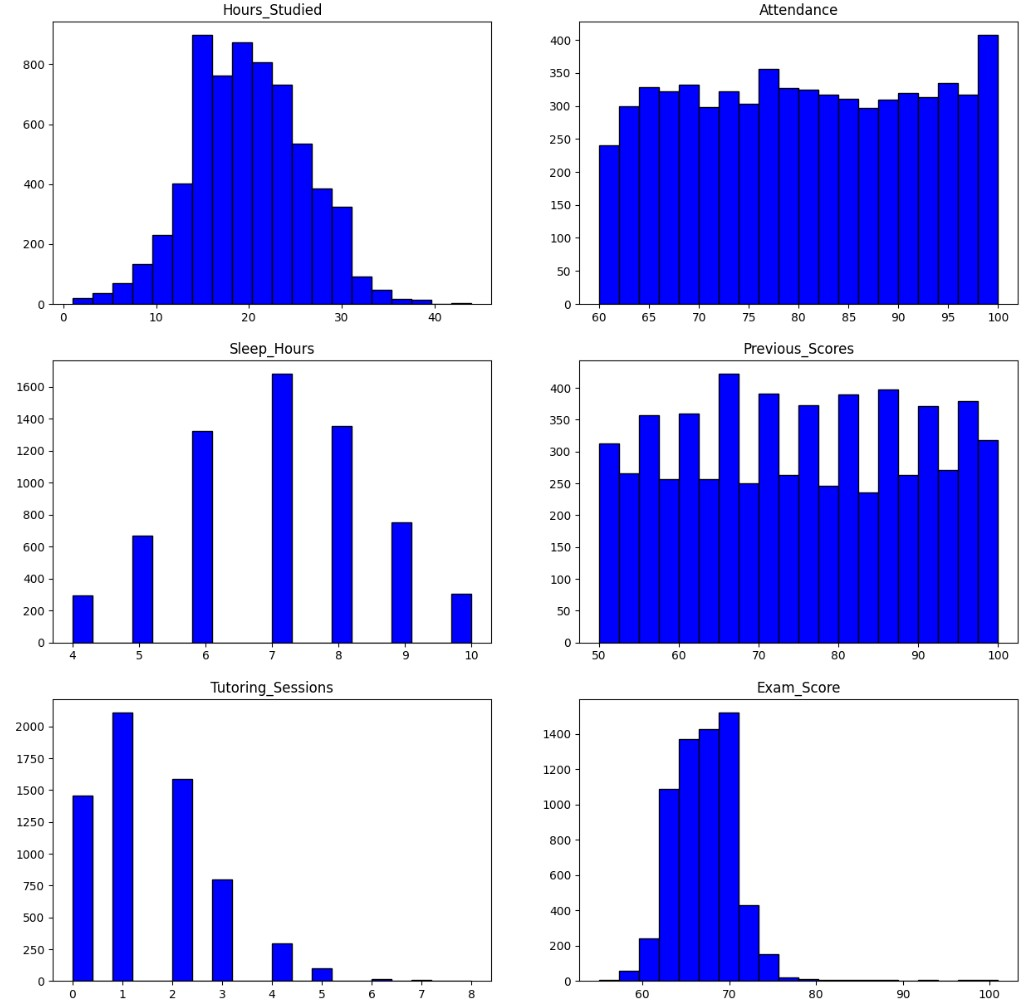
\includegraphics[width=0.9\textwidth]{./images/icon2.jpg}
    
\end{center}

Εύκολα μπορούμε να παρατηρήσουμε πως εφαρμόζουμε Standard Scaler στα χαρακτηριστικά Hours Studied και Sleep Hours αφού όπως μπορούμε να δούμε ακολουθούν κατά προσέγγιση κανονική κατανομή, MinMax Scaler στα χαρακτηριστικά Attendance και Previous Scores αφού προσεγγίζουν την ομοιόμορφη κατανομή και Robust Scaler στο χαρακτηριστικό Tutoring Sessions αφού όπως μπορούμε να δούμε περιέχει ακραίες τιμές. Η μεταβλητή στόχος Exam Scores δεν χρειάζεται να κλιμακωθεί αφού αποτελεί την εξαρτημένη μεταβλητή του μοντέλου μας.\\
\\
\noindent Οι σχέσεις για κάθε τύπο κλιμάκωσης δίνονται παρακάτω: 

\section*{Μέθοδοι Κλιμάκωσης}

\subsection*{StandardScaler}
Η μετατροπή με τη μέθοδο StandardScaler ορίζεται ως:
\[
X' = \frac{X - \mu}{\sigma}
\]
όπου:
\begin{itemize}
    \item \( X \): Η τιμή της παρατήρησης στο χαρακτηριστικό.
    \item \( \mu \): Ο μέσος όρος του χαρακτηριστικού.
    \item \( \sigma \): Η τυπική απόκλιση του χαρακτηριστικού.
\end{itemize}

\noindent Ο Standard Scaler μετασχηματίζει τα δεδομένα έτσι ώστε να έχουν μέση τιμή ίση με 0 και τυπική απόκλιση ίση με 1.

\subsection*{MinMaxScaler}
Η μετατροπή με τη μέθοδο MinMaxScaler ορίζεται ως:
\[
X' = \frac{X - X_{\text{min}}}{X_{\text{max}} - X_{\text{min}}}
\]
όπου:
\begin{itemize}
    \item \( X \): Η τιμή της παρατήρησης στο χαρακτηριστικό.
    \item \( X_{\text{min}} \): Η ελάχιστη τιμή του χαρακτηριστικού.
    \item \( X_{\text{max}} \): Η μέγιστη τιμή του χαρακτηριστικού.
\end{itemize}

\noindent Ο MinMax Scaler κλιμακώνει τα δεδομένα σε μια καθορισμένη περιοχή, συνήθως [0,1].



\subsection*{RobustScaler}
Η μετατροπή με τη μέθοδο RobustScaler ορίζεται ως:
\[
X' = \frac{X - Q_2}{Q_3 - Q_1}
\]
όπου:
\begin{itemize}
    \item \( X \): Η τιμή της παρατήρησης στο χαρακτηριστικό.
    \item \( Q_2 \): Η διάμεσος (median) του χαρακτηριστικού.
    \item \( Q_1 \): Το πρώτο τεταρτημόριο (25η εκατοστιαία θέση).
    \item \( Q_3 \): Το τρίτο τεταρτημόριο (75η εκατοστιαία θέση).\\
\end{itemize}

\noindent Ο Robust scaler μετασχηματίζει τα δεδομένα έτσι ώστε να έχουν κέντρο την διάμεσο η οποία γίνεται ίση με 0 και να μειώσει την επίδραση των ακραίων τιμών.\\

\noindent Γνωρίζουμε πως τα μοντέλα μηχανικής μάθησης δεν μπορούν να διαχειριστούν μη αριθμητικά δεδομένα. Επομένως, μέσω των encoders θα τα μετατρέψουμε με κατάλληλο τρόπο σε αριθμητικά χωρίς όμως να αλλάζουμε την κατηγορική τους ιδιότητα. Θα χρησιμοποιήσουμε Ordinal encoder για τα χαρακτηριστικά τα οποία περιέχουν κατηγορίες, οι οποίες έχουν κάποια φυσική σειρά(π.χ. "Low","Medium","High") και OneHot encoder για τα χαρακτηριστικά τα οποία περιέχουν κατηγορίες, οι οποίες δεν έχουν κάποια φυσική σειρά(π.χ. "Yes","No"). Επομένως τα κατηγορικά χαρακτηριστικά "Parental Involvement","Access to Resources","Motivation Level","Family Income", "Teacher Quality","Parental Education Level", "Distance from Home" και "Physical Activity" κωδικοποιούνται με ordinal encoding ενώ τα υπόλοιπα κατηγορικά χαρακτηριστικά με Onehot.

Η μέθοδος orindal encoding κωδικοποιεί με αριθμητικές τιμές κάθε κατηγορία με βάση την σειρά ή την θέση τους ξεκινώντας απο το 0. Για παράδειγμα εάν έχουμε τις κατηγορίες "Low","Medium","High" θα τους αναθέσει τις τιμές 0,1,2 αντίστοιχα. 

Η μέθοδος onehot encoding διαγράφει την κατηγορική στήλη και δημιουργεί για κάθε κατηγορία μια νέα που για κάθε παρατήρηση περιέχει την τιμή 1 αν το δείγμα ανήκει σε αυτήν την κατηγορία και 0 διαφορετικά. 
\subsection{Επιλογή χαρακτηριστικών}

Η επιλογή των χαρακτηριστικών που θα χρησιμοποιήσουμε για την πρόβλεψη του στόχου αποτελέι σημαντικό βήμα. Απο την μια προσπαθούμε να επιλέξουμε όλα τα σημαντικά χαρακτηριστικά έτσι ώστε να αποφύγουμε την υποπροσαρμογή, δηλαδή το μοντέλο μας να μην έχει τις απαραίτητες πληροφορίες για να αποτυπώσει την σχέση μεταξύ των δεδομένων και της μεταβλητής στόχου και απο την άλλη προσπαθούμε να επιλέξουμε όσο το δυνατό λιγότερα μη σημαντικά χαρακτηριστικά έτσι ώστε να αποφύγουμε την υπερπροσαρμογή, δηλαδή το μοντέλο μας να αποδίδει πολύ καλά στα δεδομένα εκπαίδευσης αλλά να αδυνατεί να γενικεύσει σε νέα δεδομένα.Αρχικά θα ορίσουμε 8 στο σύνολο μοντέλα παλινδρόμισης για τα οποία θα εξετάσουμε την απόδοση τους μέσω μιας μετρικής για κάθε συνδυασμό χαρακτηριστικών. Τα μοντέλα παλινδρόμισης τα οποία θα εξετάσουμε είναι τα εξής:\\
\begin{enumerate}
    \item Πολυωνιμικό μοντέλο παλινδρόμισης
    \item Γραμμική παλινδρόμιση
    \item Decision Tree παλινδρόμιση
    \item Random Forest παλινδρόμιση
    \item Support Vector παλινδρόμιση
    \item Gradient Boosting παλινδρόμιση
    \item Παλινδρόμιση Ridge
    \item Παλινδρόμιση Lasso\\
\end{enumerate}

 Για την πραγματοποίηση της παραπάνω διαδικασίας θα χρησιμοποιήσουμε τον αλγόριθμο Sequential feature selection (SFS). Θα μπορούσαμε να κάνουμε την διαδικασία αυτή και μέσω των πινάκων συσχέτισης Pearson, Cramer's V και ANOVA διαγράφοντας για κάθε ζεύγος μεταβλητών με ισχυρή συσχέτιση την μια απο τις δύο μεταβλητές αλλά με την διαφορά πως δεν θα είχαμε τόσο καλά αποτελέσματα όσο με την μέθοδο SFS. Η μέθοδος SFS με επιλογή για backwards selection ξεκινά με το πλήρες σύνολο χαρακτηριστικών. Το σύνολο εκπαίδευσης χωρίζεται σε k=cross-validation ίσα μέρη(folds). Σε κάθε επανάληψη, αφαιρείται ένα χαρακτηριστικό από το τρέχον σύνολο και το μοντέλο εκπαιδεύεται χρησιμοποιώντας τα εναπομείναντα χαρακτηριστικά. Το μοντέλο εκπαιδεύεται k φορές, χρησιμοποιώντας κάθε φορά ένα διαφορετικό fold ως σύνολο δοκιμής (test set), ενώ τα υπόλοιπα k-1 folds χρησιμοποιούνται ως σύνολο εκπαίδευσης (training set). Η απόδοση για κάθε αφαίρεση χαρακτηριστικού αξιολογείται με βάση τον μέσο όρο της απόδοσης για κάθε επιλογή fold ώς test set χρησιμοποιώντας κάποιο προκαθορισμένο κριτήριο, όπως το μέσο τετραγωνικό σφάλμα (MSE). Το χαρακτηριστικό που οδηγεί στη μικρότερη μείωση της απόδοσης αφαιρείται οριστικά από το σύνολο. Η διαδικασία συνεχίζεται μέχρι να επιτευχθεί ο επιθυμητός αριθμός χαρακτηριστικών. Για κάθε ένα απο τα μοντέλα παλινδρόμισης που αναφέραμε παραπάνω εντοπίσαμε τα χαρακτηριστικά τα οποία οδηγούν στο μικρότερο μέσο τετραγωνικό σφάλμα. Για την καλύτερη κατανόηση της μεθόδου, παρουσιάζεται παρακάτω η γραφική παράσταση του βέλτιστου αρνητικού μέσου τετραγωνικού σφάλματος. Η γραφική αφορά το μοντέλο παλινδρόμισης Decision Tree και βασίζεται στα χαρακτηριστικά που ελαχιστοποιούν το μέσο τετραγωνικό σφάλμα. Συγκεκριμένα, η γραφική απεικονίζει τη σχέση μεταξύ των χαρακτηριστικών όπως αυτά επιλέχθηκαν μέσω της συγκεκριμένης μεθόδου και του αρνητικού μέσου τετραγωνικού σφάλματος.

\begin{center}
    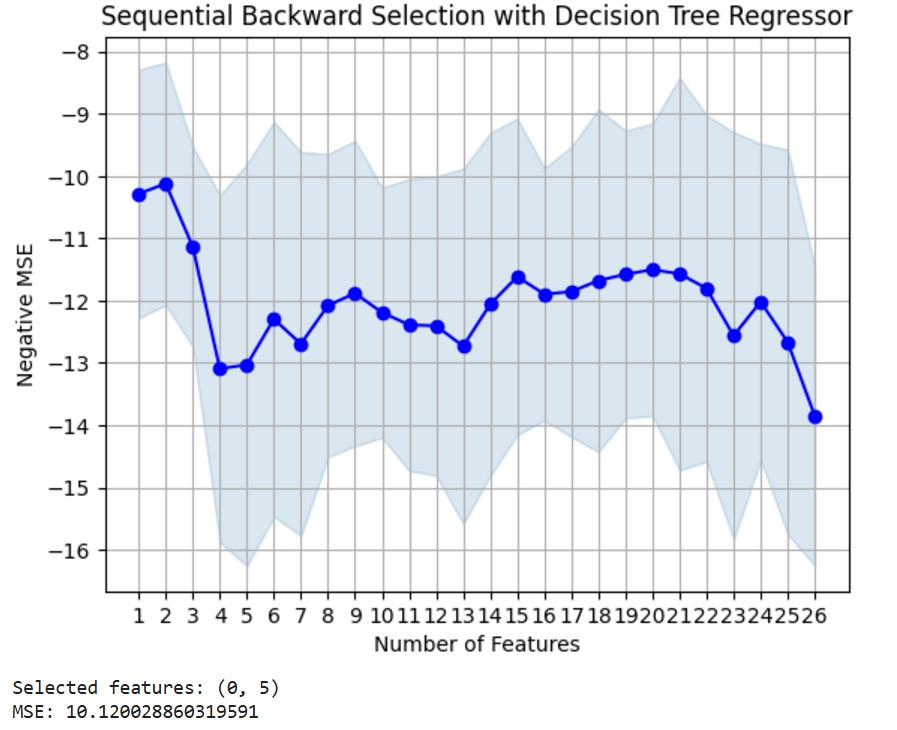
\includegraphics[width=0.9\textwidth]{./images/icon8.jpg}
    
\end{center}

Μπορούμε εύκολα να παρατηρήσουμε πως το το μεγαλύτερο αρνητικό μέσο τετραγωνικό σφάλμα επιτυγχάνετε για αριθμό χαρακτηριστικών ίσο με 2. Το αντίστοιχο καλύτερο μέσο τετραγωνικό σφάλμα είναι ίσο με 10.12 και επιτυγχάνετε χρησιμοποιώντας την πρώτη και έκτη στήλη του πίνακα δεδομένων.

\subsection{Επιλογή υπερπαραμέτρων}
Για κάθε ένα από τα μοντέλα παλινδρόμησης που ορίσαμε παραπάνω, πραγματοποιήσαμε βελτιστοποίηση υπερπαραμέτρων (hyperparameter tuning) χρησιμοποιώντας τη μέθοδο GridSearchCV. Η βελτιστοποίηση έγινε για κάθε μοντέλο παλινδρόμισης χρησιμοποιώντας τα αντίστοιχα χαρακτηριστικά που επιλέχθηκαν ως βέλτιστα μέσω της μεθόδου Sequential Forward Selection (SFS). Στη διαδικασία, θέσαμε cross-validation = 10 και επιλέξαμε ως μετρική απόδοσης το μέσο τετραγωνικό σφάλμα(MSE). Η διαδικασία βελτιστοποίησης πραγματοποιήθηκε σε δύο στάδια. Aρχικά, εξετάσαμε ένα εύρος παραμέτρων γύρω από τις προεπιλεγμένες τιμές (default parameters), ώστε να αποκτήσουμε μια αρχική εικόνα για τη συμπεριφορά του μοντέλου. Στη συνέχεια, εστιάσαμε στις παραμέτρους που ανέδειξε η πρώτη διαδικασία ως πιο σημαντικές, προσαρμόζοντας το εύρος των τιμών τους για πιο λεπτομερή αναζήτηση. Με αυτόν τον τρόπο καταφέραμε να βελτιώσουμε περαιτέρω την απόδοση των μοντέλων μας, εξασφαλίζοντας καλύτερα αποτελέσματα.

Η μέθοδος GridSearchCV λειτουργεί ώς ακολούθως.
Το σύνολο εκπαίδευσης χωρίζεται σε k=cross-validation ίσα μέρη(folds). Στη συνέχεια, για κάθε συνδυασμό υπερπαραμέτρων που ορίζει ο χρήστης το μοντέλο εκπαιδεύεται k φορές, χρησιμοποιώντας κάθε φορά ένα διαφορετικό fold ως σύνολο δοκιμής (test set), ενώ τα υπόλοιπα k-1 folds χρησιμοποιούνται ως σύνολο εκπαίδευσης(training set). Η απόδοση κάθε συνδυασμού υπερπαραμέτρων αξιολογείται με βάση τον μέσο όρο της απόδοσης για κάθε επιλογή fold ώς test set. Τέλος, επιλέγεται ο συνδυασμός υπερπαραμέτρων που βελτιστοποιεί τη μετρική απόδοσης.
\subsection{Επιλογή μοντέλου}
Για να βρούμε το τελικό βέλτιστο μοντέλο παλινδρόμισης απο αυτά που εξετάσαμε κατασκευάσαμε το ραυδόγραμμα του μέσου τετραγωνικού σφάλματος για κάθε ένα απο τα μοντέλα παλινδρόμισης που βελτιστοποιήσαμε. Το ραυδόγραμμα αυτό παρουσιάζεται παρακάτω: 

\begin{center}
    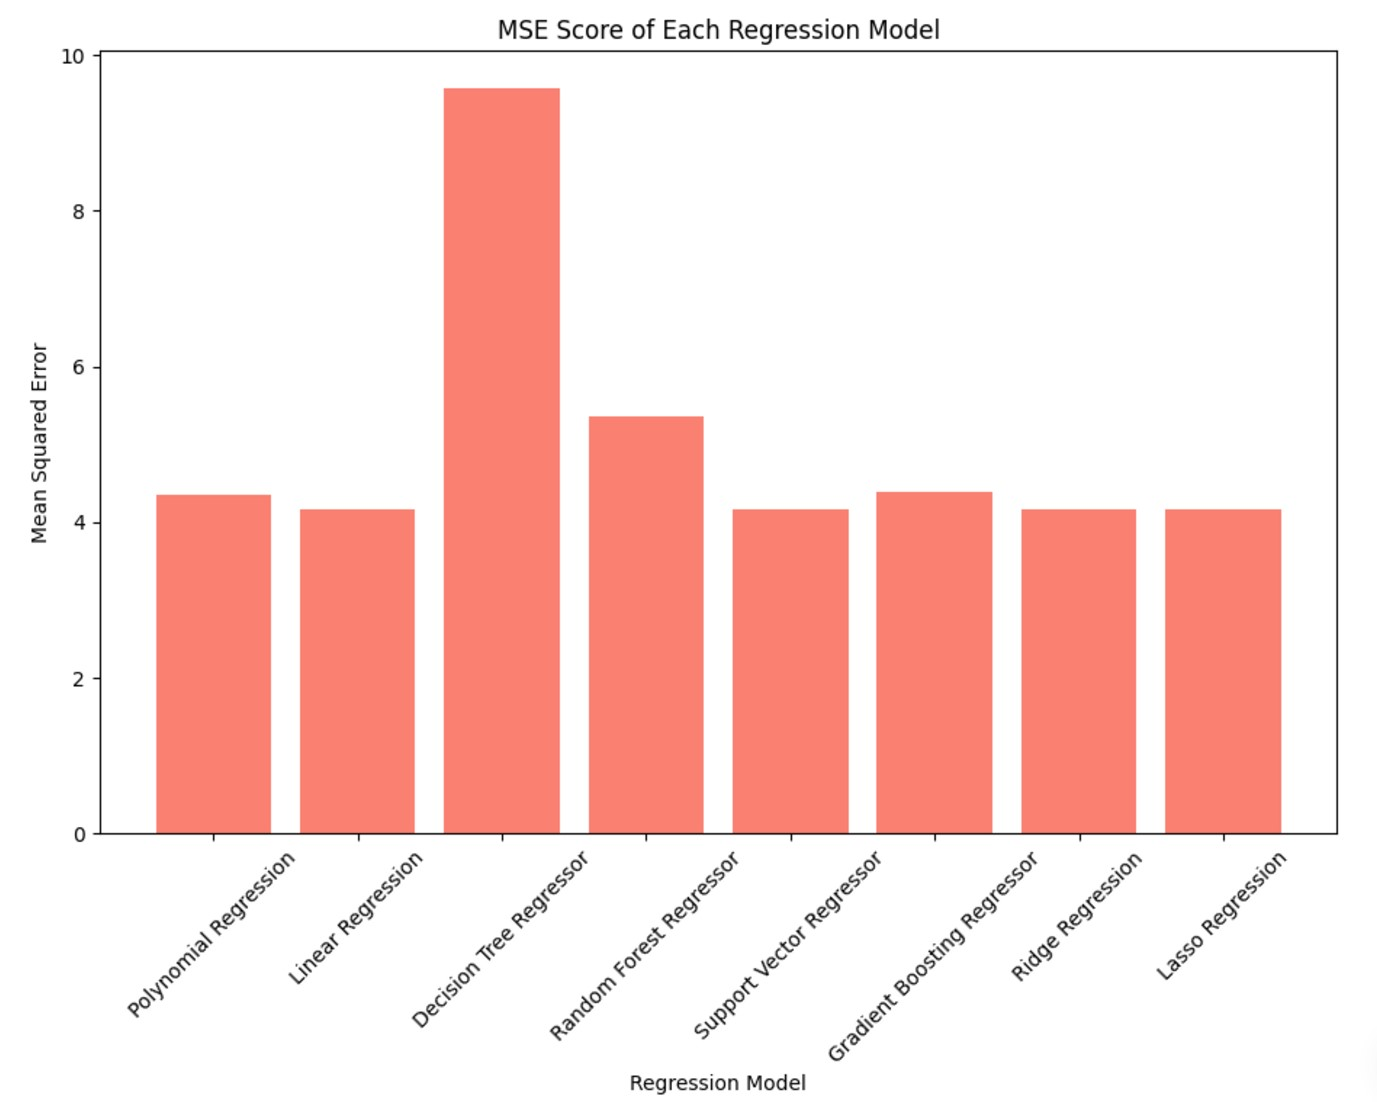
\includegraphics[width=0.9\textwidth]{./images/icon9.jpg}
    
\end{center}

Το μοντέλο το οποίο περιγράφει καλύτερα τα δεδομένα μας και προβλέπει σε καλύτερο βαθμό τον βαθμό του μαθητή με βάση την μετρική απόδοσης MSE είναι το μοντέλο παλινδρόμισης Lasso με μέσο τετραγωνικό σφάλμα ίσο με 4.155, επομένως έχουμε RMSE=\(\sqrt{MSE}=2.038\) και αυτό σημαίνει πως κατά μέσο όρο η πρόβλεψη μας για κάθε βαθμό εξέτασης διαφέρει κατά 2.038 μονάδες απο την πραγματική τιμή. Με βάση την ανάλυση που κάναμε για τις υπερπαραμέτρους θέσαμε ρυθμό κανονικοποίησης (α) ίσο με 0.0001, μέγιστο αριθμό επαναλήψεων(max\_iter) ίσο με 500 και ανοχή σύγκλισης(tol) ίση με 0.1.Για να εξετάσουμε περαιτέρω την απόδοση του μοντέλου μας υπολογίσαμε τον συντελεστή προσδιορισμού \( R^2 \), ο οποίος ισούται με 0.733  επομένως το μοντέλο μας εξηγά το 73.3\(\%\) της μεταβλητότητας του βαθμού του μαθητή(Exam Score). Τέλος, κατασκευάσαμε το γράφημα που φαίνετε παρακάτω όπου παρουσιάζει τις προβλεπόμενες τιμές του συνόλου δοκιμής σε σχέση με τις αντίστοιχες πραγματικές τιμές. 


\begin{center}
    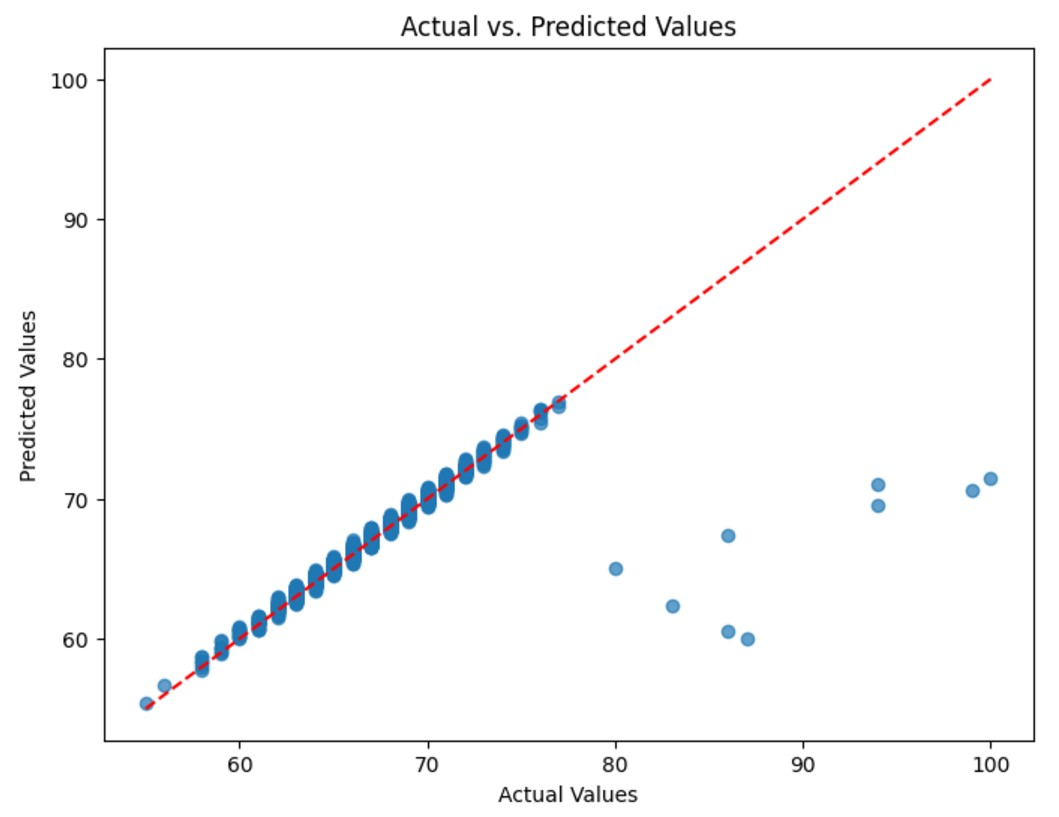
\includegraphics[width=0.89\textwidth]{./images/icon10.jpg}
    
\end{center}

Μπορούμε να παρατηρήσουμε πως το μοντέλο μας με βάση την παραπάνω γραφική παράσταση υπολογίζει σε αρκετά ικανοποιητικό βαθμό τον βαθμό του μαθητή για τιμές μικρότερες απο 80. Για τιμές μεγαλύτερες απο 80 δεν μπορούμε να πούμε το ίδιο. Αυτό οφείλετε στο ότι δεν υπάρχουν αρκετοί μαθητές οι οποίοι πήραν βαθμό μεγαλύτερο απο 80 στο training set (35 σε αριθμό), επομένως το μοντέλο μηχανικής μάθησης που δημιουργήσαμε δεν έχει αρκετά δεδομένα για να προβλέψει ικανοποιητικά τον τελικό βαθμό του μαθητή. Επίσης λόγω της μεγάλης διαφοράς στο πλήθος των δεδομένων στο training set για βαθμούς μικρότερους απο 80 σε σχέση με μεγαλύτερους απο αυτό, μπορεί να οδήγησε το μοντέλο μας σε υπερβολική εστίαση στα δεδομένα μικρότερα απο 80(biased ώς πρός αυτά τα δεδομένα) αφού τελικά θα οδηγούσε σε μικρότερο μέσο τετραγωνικό σφάλμα σε αντίθεση με το να το έκανε γενίκευση(generalize) και για τιμές μεγαλύτερες απο 80.

\newpage
\section{Το μοντέλο παλινδρόμισης Lasso}
\subsection{Έγκριση ειδικού πλαισίου χωροταξικού σχεδιασμού}
Αναλύεται η διαδικασία έγκρισης του πλαισίου.

\subsection{Καθορισμός περιοχών αιολικής προτεραιότητας}
Αναλύονται οι παράγοντες επιλογής περιοχών.

\subsection{Παράμετροι που καθορίζουν τις αποστάσεις}
Παρουσιάζονται τα κριτήρια για τις αποστάσεις υποδομών.

\newpage
\section{Σύγκριση με έρευνες}
\subsection{Επεξήγηση των παραμέτρων}
 Καταρχάς για να μπορούμε να κάνουμε την σύγκριση μεταξύ συγκεκριμένων ερευνών που υπάρχουν
 διαθέσιμες στο ευρύκοινόκαιτωναποτελεσμάτωνπουπροέκυψανμέσωτηςδικήςμαςανάλυσης,πρέπει
 πρώτα να κάνουμε μια ανάλυση της σχέσης μεταξύ του τελικού βαθμού του μαθητή και των διάφορων
 ανεξάρτητων μεταβλητών. \\
 
\noindent  Μέσω του μοντέλου μηχανικής μάθησης που δημιουργήσαμε πήραμε τα παρακάτω αποτελέσματα: \\

\begin{table}[ht]
\centering
\begin{tabular}{lrr}
\toprule
\textbf{Feature} & \textbf{Coefficient} \\
\midrule
Attendance                    & 7.945534e+00 \\
Previous\_Scores              & 2.432289e+00 \\
Tutoring\_Sessions            & 4.838539e-01 \\
Hours\_Studied                & 1.769307e+00 \\
Parental\_Involvement         & 1.006635e+00 \\
Access\_to\_Resources         & 1.021990e+00 \\
Motivation\_Level             & 5.513339e-01 \\
Family\_Income                & 5.666131e-01 \\
Teacher\_Quality              & 5.520568e-01 \\
Parental\_Education\_Level    & 4.946623e-01 \\
Distance\_from\_Home          & -4.593309e-01 \\
Physical\_Activity            & 1.992808e-01 \\
Extracurricular\_Activities\_No & -5.626076e-01 \\
Extracurricular\_Activities\_Yes & 1.337722e-16 \\
Internet\_Access\_No          & -8.974091e-01 \\
Peer\_Influence\_Negative     & -8.970209e-01 \\
Peer\_Influence\_Neutral      & -3.381165e-01 \\
Peer\_Influence\_Positive     & 1.176801e-01 \\
Learning\_Disabilities\_No    & 8.672434e-01 \\
\midrule
\textbf{Intercept} & \textbf{57.07844535052128} \\
\bottomrule
\end{tabular}
\label{tab:coefficients}
\end{table}

\noindent Εύκολα μπορούμε να συμπεράνουμε πως:\\

\begin{enumerate}
    \item \textbf{Parental Involvement} Ο βαθμός εμπλοκής των γονέων στην εκπαίδευση του μαθητή αναμένετε
 να συμβάλλει θετικά στον βαθμό του μαθητή. Συγκεκριμένα κατηγοριοποιείται σε τρία επίπεδα:
 ’Low’, ’Medium’ και ’High’. Για κάθε μεταβολή κατά ένα επίπεδο, από ’Low’ σε ’Medium’ ή
 από ’Medium’ σε ’High’, ο βαθμός του μαθητή αναμένετε να αυξηθεί κατά μία περίπου μονάδα.
 
 	\item \textbf{Access to Resources} Η πρόσβαση του μαθητή σε εκπαιδευτικό υλικό αναμένετε να συμβάλλει
 θετικά στον βαθμό του μαθητή. Συγκεκριμένα κατηγοριοποιείται σε τρία επίπεδα: ’Low’,’Medium’
 και ’High’. Για κάθε μεταβολή κατά ένα επίπεδο, από ’Low’ σε ’Medium’ ή από ’Medium’ σε
 ’High’, ο βαθμός του μαθητή αναμένετε να αυξηθεί κατά περίπου 1.02 μονάδες.
 
 \item \textbf{Motivation Level} Το κίνητρο του μαθητή συμβάλλει αναμένετε να συμβάλλει θετικά στον βαθμό
 του μαθητή. Συγκεκριμένα κατηγοριοποιείται σε τρία επίπεδα: ’Low’, ’Medium’ και ’High’. Για
 κάθε μεταβολή κατά ένα επίπεδο, από ’Low’ σε ’Medium’ ή από ’Medium’ σε ’High’, ο βαθμός
 του μαθητή αναμένετε να αυξηθεί κατά περίπου 0.55 μονάδες.
 
 \item \textbf{FamilyIncome} Το οικογενειακό εισόδημα του μαθητή αναμένετε νασυμβάλλει θετικά στον βαθμό
 του μαθητή. Συγκεκριμένα κατηγοριοποιείται σε τρία επίπεδα: ’Low’, ’Medium’ και ’High’. Για
 κάθε μεταβολή κατά ένα επίπεδο, από ’Low’ σε ’Medium’ ή από ’Medium’ σε ’High’, ο βαθμός
 του μαθητή αναμένετε να αυξηθεί κατά περίπου 0.57 μονάδες.
 
 \item \textbf{Teacher Quality} Η εκπαιδευτική ικανότητα του καθηγητή του μαθητή αναμένετε να συμβάλλει
 θετικά στον βαθμό του μαθητή. Συγκεκριμένα κατηγοριοποιείται σε τρία επίπεδα: ’Low’,’Medium’
 και ’High’. Για κάθε μεταβολή κατά ένα επίπεδο, από ’Low’ σε ’Medium’ ή από ’Medium’ σε
 ’High’, ο βαθμός του μαθητή αναμένετε να αυξηθεί κατά περίπου 0.55 μονάδες.
 
 \item \textbf{Parental Education Level} Το επίπεδο εκπαίδευσης του γονέα του μαθητή αναμένετε να συμβάλλει
 θετικά στον βαθμό του μαθητή. Συγκεκριμένα κατηγοριοποιείται σε 3 επίπεδα: ’High School’,
 ’College’ και ’Postgraduate’. Για κάθε μεταβολή κατά ένα επίπεδο, από ’High School’ σε ’Col
lege’ ή από ’College’ σε ’Postgraduate’, ο βαθμός του μαθητή αναμένετε να αυξηθεί κατά περίπου
 0.49 μονάδες.
 
 \item \textbf{Distance from Home} Η απόσταση του σχολείου απο το σπίτι του μαθητή αναμένετε να συμβάλλει
 αρνητικά στον βαθμό του μαθητή. Συγκεκριμένα κατηγοριοποιείται σε τρία επίπεδα: ’Near’,
 ’Moderate’ και ’Far’. Για κάθε μεταβολή κατά ένα επίπεδο, από ’Near’ σε ’Moderate’ ή από
 ’Moderate’ σε ’Far’, ο βαθμός του μαθητή αναμένετε να μειωθεί κατά περίπου 0.46 μονάδες.
 
 \item \textbf{Physical Activity} Το επίπεδο φυσικής δραστηριότητας του μαθητή αναμένετε να συμβάλλει θετικά
 στον βαθμό του μαθητή. Συγκεκριμένα κατηγοριοποιείται σε 7 επίπεδα: ’Sedentary’, ’Light’,
 ’Moderate’, ’Active’, ’Very Active’, ’Highly Active’ και ’Athlete’. Για κάθε μεταβολή κατά ένα
 επίπεδο, από ’Sedentary’ σε ’Light’, από ’Light’ σε ’Moderate’ κ.ο.κ. , ο βαθμός του μαθητή
 αναμένετε να αυξηθεί κατά περίπου 0.2 μονάδες.

 \item \textbf{Peer Influence}  Η μορφή της επιρρόης που δέχεται ο μαθητής απο ομήλικους του επιρεάζει και
 τον βαθμό του. Συγκεκριμένα η επιρροή αυτή χωρίζετε σε 3 κατηγορίες ’Negative’, ’Neutral’ και
 ’Positive’. Για μεταβολή αυτού απο ’Negative’ σε ’Neutral’, ο βαθμός του μαθητή αναμένετε να
 αυξηθεί κατά περίπου 0.56 μονάδες. Για μεταβολή αυτού απο ’Neutral’ σε ’Positive’, ο βαθμός
 του μαθητή αναμένετε να αυξηθεί κατά περίπου 0.46 μονάδες.
    
    \item \textbf{Extracurricular Activities}  Η συμμετοχή του μαθητή σε εξωσχολικές δραστηριότητες αναμένετε
 να συμβάλλει θετικά στον βαθμό του μαθητή. Συγκεκριμένα εάν ο μαθητής συμμετέχει σε εξωσχολικές
 δραστηριότητες ο βαθμός του αναμένετε να αυξηθεί κατά περίπου 0.56 μονάδες.
 
 \item \textbf{Internet Access}  Η πρόσβαση του μαθητή στο διαδύκτιο αναμένετε να συμβάλλει θετικά στον
 βαθμό του μαθητή. Συγκεκριμένα εάν ο μαθητής έχει πρόσβαση στο διαδίκτυο ο βαθμός του
 αναμένετε να αυξηθεί κατά περίπου 0.90 μονάδες.
 
 \item \textbf{Learning Disabilities} Η ύπαρξη μαθησιακών δυσκολιών στον μαθητή αναμένετε να συμβάλλει
 αρνητικά στον βαθμό του. Συγκεκριμένα εάν ο μαθητής έχει μαθησιακές δυσκολίες ο βαθμός του
 αναμένετε να μειωθεί κατά περίπου 0.87 μονάδες.\\
\end{enumerate}

\noindent Η επεξήγηση των μεταβολών για κάθε χαρακτηριστικό το οποίο παίρνει αριθμητικές τιμές θέλει
 προσοχή. Αυτό οφείλετε στο ότι τα βάρη που υπολογίσαμε δείχνουν την μεταβολή του βαθμού του
 μαθητή όχι για τις μεταβλητές Attendance, Previous Scores , Tutoring Sessions και Hours Studied
 αλλά για τις κλιμακωμένες τιμές τους. Για να βρούμε την πραγματική τους σχέση θα κινηθούμε
 ώς ακολούθως:\\
 
 \begin{itemize}
    \item Εάν το χαρακτηριστικό κλιμακώθηκε μέσω Standard Scaler(Συγκεκριμένα η Hours Studied) ,τότε για κάθε μεταβολή κατά μια μονάδα του χαρακτηριστικού αυτού θα έχουμε μεταβολή του βαθμού του μαθητή κατά coeff/std(feature) μονάδες, όπου coeff η αντίστοιχη τιμή του coefficient του χαρακτηριστικού όπως φαίνετε στον πίνακα παραπάνω και std(feature) η τυπική του απόκλιση που προκύπτει απο τα δεδομένα.
    
    \item Εάν το χαρακτηριστικό κλιμακώθηκε μέσω MinMax Scaler(Συγκεκριμένα οι Attendance και Previous Scores) ,τότε για κάθε μεταβολή κατά μια μονάδα του χαρακτηριστικού αυτού θα έχουμε μεταβολή του βαθμού του μαθητή κατά coeff/(max(feature)-min(feature)) μονάδες, όπου coeff η αντίστοιχη τιμή του coefficient του χαρακτηριστικού όπως φαίνετε στον πίνακα παραπάνω, min(feature) η ελάχιστη τιμή του χαρακτηριστικού αυτού στα δεδομένα και max(feature) η μέγιστη τιμή του χαρακτηριστικού στα δεδομένα.
    
     \item Εάν το χαρακτηριστικό κλιμακώθηκε μέσω Robust Scaler(Συγκεκριμένα η Tutoring Sessions) ,τότε για κάθε μεταβολή κατά μια μονάδα του χαρακτηριστικού αυτού θα έχουμε μεταβολή του βαθμού του μαθητή κατά coeff/IQR(feature) μονάδες, όπου coeff η αντίστοιχη τιμή του coefficient του χαρακτηριστικού όπως φαίνετε στον πίνακα παραπάνω και IQR(feature) το ενδοτεταρτημοριακό του εύρος που προκύπτει απο τα δεδομένα.
  \end{itemize}
  
\noindent Μέσω της ανάλυσης που κάναμε πήραμε τα παρακάτω διαγράμματα που δείχνουν την σχέση μεταξύ των ποσοτικών χαρακτηριστικών και του βαθμού του μαθητή: \\

\begin{center}
    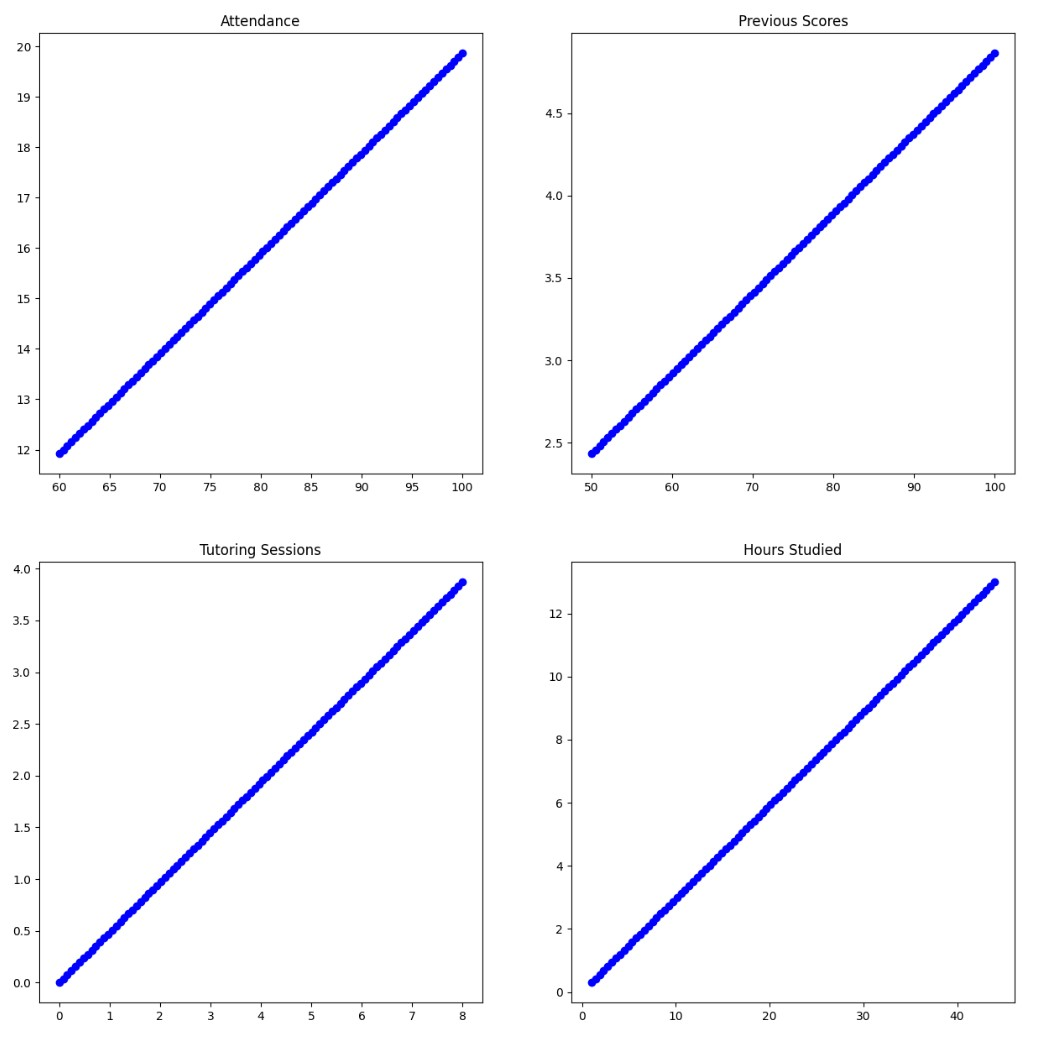
\includegraphics[width=0.89\textwidth]{./images/icon12.jpg}
    
\end{center}

Εύκολα μπορούμε να συμπεράνουμε πως: \\

\begin{enumerate}
    \item \textbf{Attendance} Το ποσοστό της προσέλευση του μαθητή στο μάθημα αναμένετε
 να συμβάλλει στον προσδιορισμό του βαθμού του μαθητή. Συγκεκριμένα η μεταβολή κατά μια μονάδα του χαρακτηριστικού αυτού αναμένετε να μεταβάλλει τον βαθμό του μαθητή κατά περίπου 0.2 μονάδες.
 
 	\item \textbf{Previous Scores} Ο μέσος όρος των βαθμών του μαθητή απο προηγούμενες εξετάσεις αναμένετε
 να συμβάλλει στον προσδιορισμό του βαθμού του μαθητή. Συγκεκριμένα η μεταβολή κατά μια μονάδα του χαρακτηριστικού αυτού αναμένετε να μεταβάλλει τον βαθμό του μαθητή κατά περίπου 0.05 μονάδες.
 
 \item \textbf{Tutoring Sessions} Ο αριθμός των φροντιστηριακών μαθημάτων ανά μήνα του μαθητή αναμένετε
 να συμβάλλει στον προσδιορισμό του βαθμού του μαθητή. Συγκεκριμένα η μεταβολή κατά μια μονάδα του χαρακτηριστικού αυτού αναμένετε να μεταβάλλει τον βαθμό του μαθητή κατά περίπου 0.48 μονάδες.
 
 \item \textbf{Hours Studied} Ο αριθμός των ωρών που διάβασε ο μαθητής μέσα στην βδομάδα αναμένετε
 να συμβάλλει στον προσδιορισμό του βαθμού του μαθητή. Συγκεκριμένα η μεταβολή κατά μια μονάδα του χαρακτηριστικού αυτού αναμένετε να μεταβάλλει τον βαθμό του μαθητή κατά περίπου 0.29 μονάδες.
 
 \end{enumerate}
\newpage
\section{Βιβλιογραφία}

\end{document}
